\documentclass{report}


\usepackage{bibgerm}
\usepackage[numbers,sort&compress]{natbib}
\usepackage{amsmath,amssymb,mathtools}
\usepackage{algpseudocode,algorithm}
\usepackage{graphicx}
\usepackage{hyperref}
\usepackage{multirow}
\usepackage[utf8]{inputenc}
\usepackage{geometry}
\usepackage{parskip}
\usepackage{paralist}
\usepackage{multicol}

\geometry{verbose,a4paper,tmargin=25mm,bmargin=25mm,lmargin=15mm,rmargin=20mm}

%% Stuff ist aus ML1. vllt brauchen wir es ja noch :D
\DeclareMathOperator*{\argmax}{arg\,max}
\DeclareMathOperator*{\argmin}{arg\,min}

\newcommand{\IndState}[1][1]{\State\hspace{10mm}}
\newcommand{\mparagraph}[1]{\paragraph{#1} \mbox{}\\}

%%%%%%%%%%%%%% includeonly %%%%%%%%%%%%%%%%%%%
% Es werden nur die Teile eingebunden, die hier
% aufgefuehrt sind!
%\include{Kapitel X}
%}um es anzuzeigen.
%%%%%%%%%%%%%%%%%%%%%%%%%%%%%%%%%%%%%%%%%%%%%%
\graphicspath{{pic/}}

\begin{document}

\tableofcontents


% einfach !TEX root = rob1.tex an den Anfang packen von chaptern
% !TEX root = rob1.tex
\chapter{Einführung}

\subsection{Begriffsbildung}

\mparagraph{Roboter}
\begin{compactitem}
    \item \textbf{Industrie}: Ein Roboter ist ein frei programmierbarer, multifunktionaler
    Manipulator mit mindenstes 3 unabhängigen Achsen, um Materialien, Teile, Werkzeuge oder
    Geräte auf programmierten, variablen Bahnen zu bewegen zur Erfüllung verschiedener Aufgaben.
    \item \textbf{Wissenschaft}: Roboter sind sensomotorische Maschinen zur Erweiterung der
    menschlichen Handlungsfähigkeit. Sie bestehen aus mechatronischen Komponenten, Sensoren und
    rechnerbasierten Kontroll- und Steuerungsfunktionen.
\end{compactitem}

\mparagraph{Robotik}
Robotik ist ein interdisziplinär ausgerichtetes Forschungsgebiet, bei dem im Mittelpunkt mechanische
Vorrichtungen und geeignete Steuereinheiten selbsttätig komplexe Aufgaben verrichten.

\subsection{Asimovsche Robotergesetze}
\begin{compactenum}
    \item Ein Roboter darf keine Menschen verletzen oder durch Untätigkeit zu Schaden kommen lassen.
    \item Ein Roboter muss den Befehlen eines Menschen gehorchen, es sei denn, solche Befehle stehen
    im Widerspruch zum ersten Gesetz
    \item Ein Robot muss seine eigene Existenz schützen, solange dieser Schutz nicht dem ersten oder
    zweiten Gesetz widerspricht.
\end{compactenum}

\subsection{Anwendungsfelder}
\mparagraph{Industrieroboter}
Ein automatisch kontrollierter, reprogrammierbarer und vielseitiger Manipulator, mit 3 oder mehr
programmierbaren Achsen, welche fix am Platz oder mobil zur industriellen automatisierten
Anwendung ist.
\mparagraph{Serviceroboter}
Roboter, der halb- oder vollautonom arbeitet, mit dem Ziel, nützliche Dienste zum Wohle von Menschen
und Einrichtung zu erledigen. Keine Aufgaben im Bereich der industriellen Produktion.
\mparagraph{,,Personal Robot''}
Roboter, der den Menschen in Sachen Bewegung, Intelligenz und Kommunikation ähnelt.

% !TEX root = rob1.tex
\section{Teilsysteme eines Roboters}

% !TEX root = rob1.tex
\chapter{Mathematische Grundlagen}

\section{Euklidischer 3D Raum}
\subsection{Basiskoordinatensystem, BKS}
3-dim. Koordinatensystem. Durch orthogonale Einheitsvektoren $\vec{e}_{X,B}, \vec{e}_{Y,B},
\vec{e}_{Z,B}$ definiert
\mparagraph{Rechtsdrehend:} $\vec{e}_{X} \times \vec{e}_{Y} = \vec{e}_{Z},\text{ }\vec{x} \times \vec{y} = \vec{z}$
\mparagraph{Linksdrehend:} $\vec{e}_{X} \times \vec{e}_{Y} = -\vec{e}_{Z},\text{ }\vec{x} \times \vec{y} = \vec{-z}$

z-Richtung und Drehrichtung mit Hilfe der Rechten Hand Regel (Daumen = z Achse)

\subsection{Definitionen}
\begin{compactitem}
    \item \textbf{Ort}: Ortsvektor vom Ursprung des BKS zum Ursprung des OKS
    \item \textbf{Orientierung}: Rotationsmatrix zur Abbildung der Einheitsvektoren des OKS auf die
    Einheitsvektoren des BKS
    \item \textbf{Lage}: Ortsvektor und Rotationsmatrx des OKS bezogen auf das BKS.
    $\vec{v} = (x,y,z,\alpha,\beta,\gamma)$
\end{compactitem}

\subsection{Freiheitsgrad und Bewegungsfreiheitsgrad}
\begin{compactitem}
    \item \textbf{Freiheitsgrad f} ist die Anzahl möglicher unabhängiger Bewegungen in Bezug auf
    das BKS. Minimale Anzahl von Translationen und Rotationen zur vollständigen Beschreibung der Lage des
    Objektes.
    \item \textbf{Bewegungsfreiheitsgrad F}: $\sum_{i}^n(F_{R_i} + F_{T_i})$
    \item F $\geq$ f
\end{compactitem}
\newpage
\section{Orientierungsbeschreibung mit 3x3 Matrix}
\subsection{Rotationsmatrizen}
\begin{align}
    R_x &= \begin{bmatrix} 1 & 0 & 0  \\ 0 &\cos \alpha& -\sin\alpha \\ 0 & \sin\alpha & \cos\alpha \end{bmatrix}\\
    R_y &= \begin{bmatrix} \cos\alpha & 0 & \sin\alpha  \\ 0 & 1 & 0 \\ -\sin\alpha & 0 & \cos\alpha \end{bmatrix}\\
    R_z &= \begin{bmatrix} \cos \alpha& -\sin\alpha& 0 \\ 0 \sin\alpha & \cos\alpha & 0 \\ 0 & 0 & 1 \end{bmatrix}
\end{align}

\subsection{Drehachse}
\begin{compactitem}
    \item \textbf{Euler Winkel}: Drehung um jeweils veränderte Achse. Jede Drehung bezieht sich auf
    das neue Koordinatensystem. Von links nach rechts
    \item \textbf{Roll, Pitch, Yaw}: Drehung um unveränderte Achse. Jede Drehung bezieht sich auf
    das BKS. Von rechts nach links
\end{compactitem}

\section{Homogene 4x4 Matrix}
\mparagraph{Rotation}
$R_x$, $R_y$, $R_z$ wie bei 3x3 nur mit $(0,0,0,1)$ Extrazeile
\mparagraph{Translation}
\begin{align}
    T_{\text{trans}} &= \begin{bmatrix}1 & 0 & 0 & 0\\0 & 1 & 0 & 0\\0 & 0 & 1 & 0\\0 & 0 & 0 & 1\end{bmatrix}
\end{align}
\mparagraph{Skalierung}
Lokal und Global
\begin{align}
    T_{\text{scale}} &= \begin{pmatrix}a & 0 & 0 & 0\\0 & b & 0 & 0\\
    0 & 0 & c & 0\\0 & 0 & 0 & 1\end{pmatrix} \begin{pmatrix}x\\y\\z\\1\end{pmatrix} = \begin{pmatrix}ax\\by\\cz\\1\end{pmatrix}
\end{align}
\begin{align}
    T_{\text{scale}} &= \begin{pmatrix}1 & 0 & 0 & 0\\0 & 1 & 0 & 0\\
    0 & 0 & 1 & 0\\0 & 0 & 0 & s\end{pmatrix} \begin{pmatrix}x\\y\\z\\1\end{pmatrix} = \begin{pmatrix}x\\y\\z\\s\end{pmatrix}
\end{align}
\subsection{Lagebeschreibung}

Beschreibung der Lage des Koordinatensystems B relativ zum Koordinatensystem A
\begin{displaymath}
    ^AH_B
\end{displaymath}
\mparagraph{Transformationsabbildung}
\begin{displaymath}
    ^AH_B: ^BP \rightarrow ^AP
\end{displaymath}
\mparagraph{Transformationsoperator}
\begin{displaymath}
    H: ^BP_1 \rightarrow ^AP_2
\end{displaymath}
\subsubsection{Verkettung}

\begin{compactitem}
    \item Lage von Objekt 1 bzgl. BKS: $^\text{BKS}H_1$
    \item Lage von Objekt 1 bzgl. Objekt 1: $^{o1}H_2$
    \item Lage von Objekt 1 bzgl. Objekt 2: $^{o2}H_3$
    \item Lage von Objekt 1 bzgl. BKS: $^\text{BKS}H_3$
\end{compactitem}

\begin{align}
     ^\text{BKS}H_3 &= ^\text{BKS}H_1 * ^{o1}H_2 * ^{o2}H_3 \\
     \text{bzw.} &\prod^n_{i=1}{}^{H_{i-1}}H_i \text{ mit } H_0 = \text{BKS}
\end{align}

\subsection{Nachteile}
\begin{compactitem}
    \item Hohe Redundanz
    \item Interpolation schwierig
\end{compactitem}

\section{Quaterionen}
\textbf{Dienen nur der Rotation, nicht der Translation!}
\mparagraph{Definition}
Ein Quaternion hat die Darstellung $q = (a,b,c,d)^T$
\begin{compactitem}
    \item $a$ ist der \textbf{Realteil}
    \item $u = (b,c,d)^T$ ist der \textbf{Imaginärteil}
\end{compactitem}
\begin{align}
    q &= a + bi + cj + dk \\
    i^2 &= j^2 = k^2 = ijk = -1 \\
    ij &= -ij = k \\
    jk &= -kj = i \\
    ik &= -ki = j
\end{align}
\begin{itemize}
    \item \textbf{Addition}: $q + r = (a_q + a_r, u_q + u_r)$
    \item \textbf{Punktprodukt/Skalarprodukt}: $q \cdot r = a_qa_r +b_qb_r + c_qc_r + d_qd_r $
    \item \textbf{Multiplikation}: $q * r = (a_q + ib_q + jc_q + kd_q) * (a_r + i_br + jc_r + kd_r)$
    \item \textbf{Konjugiertes Quaternion}: $\overline{q} = (a,-u)$
    \item \textbf{Norm}: $|q| = \sqrt{a^2+b^2+c^2+d^2}$
    \item \textbf{Multiplikatives Inverses}: $q^{-1} = \frac{\overline{q}}{|q|^2}$
\end{itemize}

\subsection{Rotation}
\begin{compactitem}
    \item Winkel $\Theta$
    \item Rotationsachse $u$
    \item zu rotierender Vektor $v$
\end{compactitem}
\begin{align}
    q &= (\frac{\cos\Theta}{2},u\frac{\sin\Theta}{2})\\
    a &= (0,v)
\end{align}
Berechne: $qa\overline{q}$
\subsection{Vorteile}
\begin{compactitem}
    \item Intuitive Darstellung von Rotationen, direkte Angabe von Drehwinkel und Achse
    \item Kompakte Darstellung
    \item Rotation um gewünschte Achse
    \item Numerische Stabilität
\end{compactitem}

\section{Duale Quaternionen}
Ersetzung der 4 Reellen werte durch Dualzahlen um Orientierung und Lage zu erhalten.
\mparagraph{Duale Zahl}
\begin{displaymath}
     d = p + \epsilon \cdot s, \text{ wobei }\epsilon^2 = 0
\end{displaymath}
mit Primärteil $p$ und Sekundärteil $s$
\mparagraph{Duales Quaternion}
\begin{displaymath}
     \text{DQ} = (d_1,d_2,d_3,d_4) \text{ mit } d_i = dp_i + \epsilon \cdot ds_i
\end{displaymath}
Der Reale Skalarteil enthält den Winkelwert $\frac{\Theta}{2}$, der imaginäre Skalarteil die
Verschiebungsgröße d. \\
Die restlichen drei Dualzahlen beschreiben eine beliebige gerichtete, normierte Gerade im Raum.

% !TEX root = rob1.tex
\chapter{Robotermodellierung}
\section{Geometrisches Model}
\mparagraph{Einsatzbereich}
\begin{compactitem}
    \item Graphische Darstellung von Körpern
    \item Ausgangspunkt der Abstandsmessung und Kollisionserkennung
    \item Grundlage zur Berechnung der Bewegungen von Körpern
    \item Grundlage zur Ermittlung der wirkenden Kräfte und Momente.
\end{compactitem}

\mparagraph{Klassifizierung}
\begin{itemize}
    \item \textbf{Raum}: 2D, 2.5D, 3D Modelle
    \item \textbf{Grundprimitive}
    \begin{compactitem}
        \item Kanten- bzw. Drahtmodelle
        \item Flächen- bzw. Oberflächenmodelle
        \item Volumenmodell
    \end{compactitem}
\end{itemize}
\section{Kinematisches Model}
\textbf{Das kinematische Modell eines Roboters beschreibt die Zusammenhänge zwischen
dem Raum der Gelenkwinkel (Roboterkoord, Konfigurationsraum) und dem Raum der
Lage des Endeffektors in Weltkoordinaten (Arbeitsraum, Kartesischer Raum.)}
\subsection{Direktes kinematisches Problem, Vorwärtskinematik}

% !TEX root = rob1.tex
\chapter{Regelung von Robotersystemen}
\textbf{Laufende Beobachtung bei der mit den gewonnenen Informationen die Stellgröße derart
verändert wird, so dass trotz Störgrößeneinwirkung die Ausgangsgröße an den gewünschten Verlauf
(Sollverlauf) angeglichen wird.}

\section{Regelkreis}
\begin{figure}[!h]
    \centering
    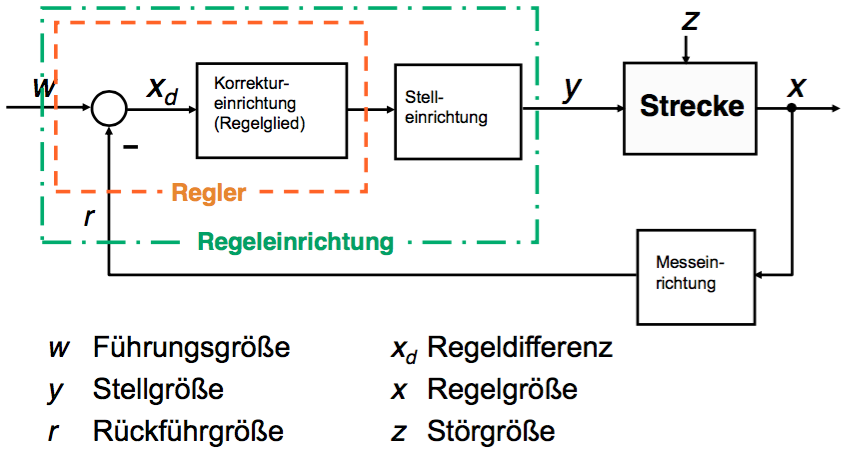
\includegraphics [scale=0.5]{regelkreis}
    \caption{Struktur eines Regelkreises}
\end{figure}

\mparagraph{Wirkungsweise}
\textbf{z} wird größer $\Rightarrow$ \textbf{x} wird gesenkt $\Rightarrow$ \textbf{r} wird abgesenkt
$\Rightarrow$ \textbf{$x_d$} wird angehoben $\Rightarrow$ \textbf{y} wird angehoben $\Rightarrow$
\textbf{x} wird angehoben mit der Tendenz den Sollwert \textbf{$x_s$} wieder anzunehmen. \\
Die Störgröße wird ausgeregelt.

\section{Grundlagen}
\subsection{Laplace Transformation}
\begin{compactitem}
    \item Rechenvereinfachung: Differential und Integralausdrücke werden zu algebraischen Ausdrücken.
    \item Gleichungslösung im Frequenzbereich statt Zeitbereich
    \item Integral muss konvergieren $\rightarrow$ lineare $f(t)$
\end{compactitem}
\begin{displaymath}
     L[f(t)] = f(s) = \int_0^\infty f(t)e^{-st}dt, s := \sigma + j\omega \text{ in } C \text{  } f(t)
      = 0, t < 0
\end{displaymath}

\begin{compactitem}
    \item \textbf{Linearitätssatz}: $L[\alpha f_i(t) + \beta f_2(t)] = \alpha f_1(s) + \beta f_2(s)$
    \item \textbf{Faltungssatz}: $L[f_1(t) * f_2(t)] = f_1(s) * f_2(s)$
    \item \textbf{Grenzwertsatz}: $f_1(t = 0) = \lim_{s \rightarrow \infty} s * f(s)$
    \item \textbf{Differentiationssatz}: $L[\frac{d}{dt}f(t)] = sF(s)$
    \item \textbf{Integrationssatz}: $L[\int f(t)dt] = \frac{1}{s}F(s)$

\end{compactitem}
\subsection{Übertragungsglieder}
\begin{compactitem}
    \item \textbf{P-Glied}: $y(t) = K * u(t)$
    \item \textbf{I-Glied}: $y(t) = K * \int_0^t u(\tau)d\tau$
    \item \textbf{D-Glied}: $y(t) = K * \dot{u}(t)$
    \item \textbf{T$_t$-Glied}: $y(t) = K * u(t-T_t)$
    \item \textbf{S-Glied}: $y(t) = K * \pm u_1(t) \pm u_2(t)$
    \item \textbf{KL-Glied}: $y(t) = K * F(u(t))$
    \item \textbf{M-Glied}: $y(t) = K * u_1(t)u_2(t)$
\end{compactitem}

\section{Reglertypen}
\subsection{PID Regler (und Unterklassen)}
\textbf{Sehr verbreitet, da für nahezu alle Prozesstypen geeignet, robust und mit geringem Aufwand
realisierbar} \\
P: güngstiges Regelverhalten, I: stationäre Genauigkeit, D: schnelle Ausregelung
\begin{align}
    u(t) = K_p (e(t) + \frac{1}{T_N}\int_o^t e(\tau)d\tau)+ T_V \frac{d}{dt}e(t))
\end{align}
mit Nachstellzeit $T_N$ und Vorhaltzeit $T_V$.

\mparagraph{Laplacetransformation}
\begin{align}
    u(t) &= K_Pe(t) + K_I \int e(t)dt + K_D \frac{d}{dt}e(t) \Leftrightarrow \\
    \Leftrightarrow u(s) &= K_Pe(s) + K_I \frac{1}{s}e(s) + K_Dse(s) \\
    \leftrightarrow \frac{u(s)}{e(s)} &= G(s) = K_P + K_I \frac{1}{s}+K_Ds \\
    \frac{\text{Ausgang}}{\text{Eingang}} &= \text{Übertragungsfunktion}
\end{align}
\subsection{Kennlinien- bzw. Kennlinienfeldregler}
\textbf{nihctlineare Übertragungsglieder}\\
z.B Zweipunktregler (Temperatur-Regelung)
\newpage
\subsection{Zustandsregler}
\textbf{Verbessertes Regelverhalten, da nicht nur die Regelabweichung, sondern im Idealfall alle
Zustandsgrößen der Regelstrecke zur Verfügung gestellt werden.} \\
regelungstechnische Behandlung von Mehrgrößensystemen, nichtlinearen und zeitvariablen
Übertragungssystemen.

\begin{figure}[!h]
    \centering
    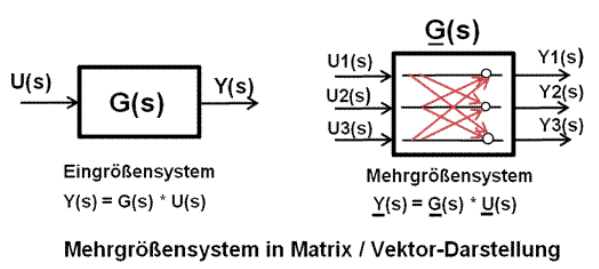
\includegraphics [scale=0.5]{mehrgroesse}
\end{figure}

\subsection{Kaskadenregelung}
\textbf{Unabhängige lineare Einzelregelkreis der einzelnen Gelenke}\\
Manipulator = Mehrgrößensystem

\begin{figure}[!h]
    \centering
    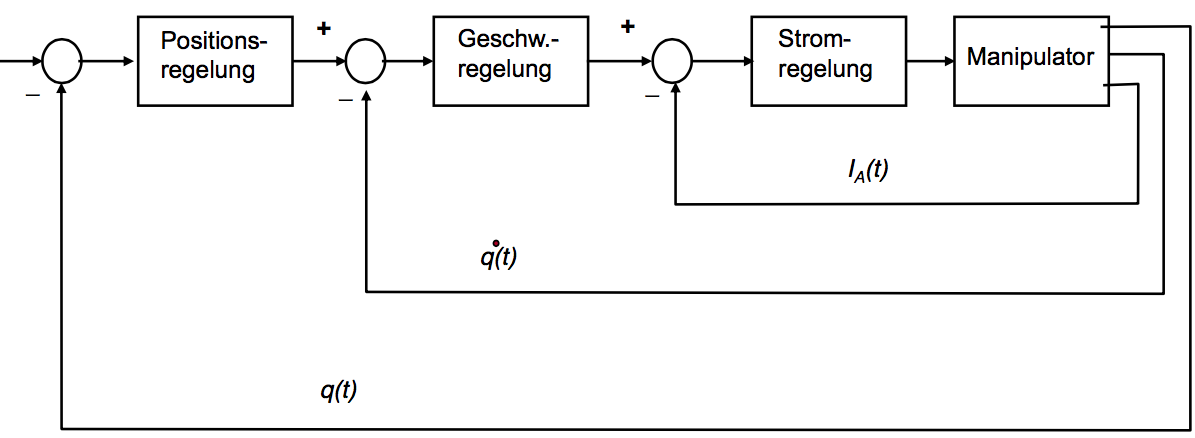
\includegraphics [scale=0.3]{kaskade}
\end{figure}

\subsection{Adaptive Regelung}
\textbf{Lageabhängige und somit zeitveränderliche Systemteile werden als Parameterschwankungen
aufgefasst}
\begin{figure}[!h]
    \centering
    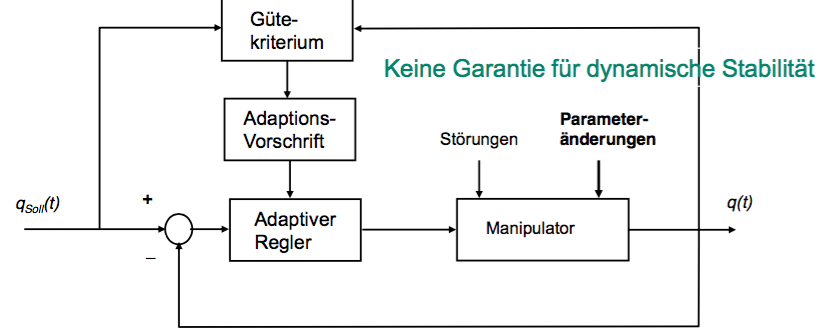
\includegraphics [scale=0.3]{adaptiv}
\end{figure}

\section{Regelungskonzepte für Manipulatoren}
\textbf{Regelung von Manipulatoren beschreibt nicht nur Positionsregelung, sondern auch die
Einbeziehung weiterer Umwelteinflüsste} (Massenträgheit des Manipulators, Gravitations-, Zentrifugal-,
Coriolis und Reibungskräfte/Momente auf die Gelenke)
\subsection{Exakte Systemmodellierung}
setzt a priori die exakte Kenntnis des Dynamikmodells und er Umgebung des Roboters voraus.
\subsection{Kraft-/Positionsregelung}
Position und Kräfte sind eng miteinander verknüpft. Steht Roboter in Kontakt mit Umgebung so bedeutet
Positionsänderung auch Kraftänderung und vice versa.

\mparagraph{Hybride Kraft-/Positionsregelung}
Wahlweise zwischen reiner Kraft und reiner Positionsregelung gewählt für jede kartesische Bewegungsrichtung
des Arms.
\mparagraph{Impedanz Regelung}
Regelt die dynamische Beziehung zwischen Kraft und Positions im Kontaktfall. \\
Idee: Interaktion Roboter-Umwelt verhält sich wie Feder-Dämpfer-Masse-System.
\begin{align}
     f(t) &= d * x(t)b * \dot{x}(t) + m * \ddot{x}(t)\\
     &\Rightarrow \text{Lapace Transformation} \Rightarrow \\
     F(s) &= (d + b+ s+ m *s ^2) * X(s)
\end{align}
Impedanz kann über Steifheit d, Dämpfung b und Trägheit m beeinflusst werden.

% !TEX root = rob1.tex
\chapter{Bahnsteuerung}

% !TEX root = rob1.tex
\chapter{Bahnplanung}

\section{Problemklassen}
\begin{itemize}
    \item \textbf{Klasse a)}
    \begin{compactitem}
        \item bekannt: vollständiges Umweltmodell und vollst. Neben-, Rand- und Zwangsbedingungen
        \item gesucht: Kollisionsfreie Bahn von Start zu Zielzustand
    \end{compactitem}
    \item \textbf{Klasse b)}
    \begin{compactitem}
        \item bekannt: unvollständiges Umweltmodell unvollst. Neben-, Rand- und Zwangsbedingungen
        \item gesucht: Kollisionsfreie Bahn von Start zu Ziel
        \item Problem: Kollision mit unbekannten Objekten
    \end{compactitem}
    \item \textbf{Klasse c)}
    \begin{compactitem}
        \item bekannt: zeitinvariantes Umweltmodell (bewegliche Hindernisse)
        \item gesucht: Kollisionsfreie Bahn von Start zu Zielzustand
        \item Problem: Hindernisse in Ort und Zeit variant
    \end{compactitem}
    \item \textbf{Klasse d)}
    \begin{compactitem}
        \item bekannt: kein Umweltmodell
        \item gesucht: Kollisionsfreie Bahn von Start zu Zielzustand
        \item Problem: Kartografie
    \end{compactitem}
    \item \textbf{Klasse e)}
    \begin{compactitem}
        \item bekannt: zeitvariantes Umweltmodell
        \item gesucht: Bahn zu einem beweglichen Ziel (Rendezvous Problem)
        \item Problem: Zielzustand in Ort und Zeit beweglich
    \end{compactitem}
\end{itemize}
\section{Definitionen}
\mparagraph{Umweltmodellierung}
\begin{compactitem}
    \item \textbf{Exakt}:Beispiel für constructed solid geometry, in Form einer
    algebraischen Beschreibung
    \item \textbf{Approximiert}: Die Umwelt wird duch Näherungen beschreiben (
    Kuben, verallgem. Zylinder, Polyeder)
\end{compactitem}

\mparagraph{Planungsalgorithmen}
\begin{compactitem}
    \item \textbf{Vollständige Verfahren}: Algorithmen liefern immer einer korrekte
    Lösung und können ermitteln, ob keine Lösung existiert
    \item \textbf{Probabilistische vollständige Verfahren}: Falls eine Lösung
    existiert konvergieren die Wahrscheinlichkeiten, dass eine Lösung gefunden
    wird bei fortschreitender Zeit gegen 1. Existiert keine Lösung, kann dies nicht
    ermittelt werden.
\end{compactitem}
\mparagraph{Konfiguration}
Eine Konfiguration q beschreibt den Zustand eines Roboters A im eukl. Raum durch Lage und Orientierung
oder im Gelenkwinkelzustandsraum durch die Werte der Gelenke.
\mparagraph{Konfigurationsraum}
Konfigurationsraum $C$ des Roboters A ist der Raum aller möglichen Konfigurationen von A
\mparagraph{Weg}
Weg für Roboter A von der Konfiguration q$_\text{Start}$ zur Konfiguration q$_\text{Ziel}$ ist eine
stetige Abbildung $\tau:[0,1] \rightarrow C$
\mparagraph{Arbeitsraumhindernis}
Arbeitsraumhindernis H ist der Raum, welcher von einem Objekt im Arbeitsraum eingenommen wird
\mparagraph{Konfigurationsraumhindernis}
$C_H$ ist die Menge aller Punkte des Konfigurationsraum, welche zu einer Kollision mit dem Hindernis
H führen
\mparagraph{Hindernisraum}
Menge aller Konfigurationsraumhindernisse $C_\text{obst} = \cup C_{H_i}$
\mparagraph{Freiraum}
Menge aller Punkte aus C, welche nicht im Hindernisraum liegen.
$C_\text{free} =  \{ q \in C | q \notin C_\text{obst}\} = C \backslash C_\text{obst}$

\section{Planungsverfahren}
\subsection{Mobile Roboter}
\begin{compactitem}
    \item Voronoi Diagramm
    \item Sichtgraph $\rightarrow$ Erweiterung der Hindernisse durch Kreis/Rechteck
    \item Zellenzerlegung
    \begin{compactitem}
        \item Exakte
        \item Approximative (Quad Tree)
    \end{compactitem}
    \item Potentialfelder mit Abstoßung und Anziehungspotentialen.
\end{compactitem}
\subsection{Manipulatoren}
\subsubsection{Probabilistic Roadmaps, PRM}
\begin{compactitem}
    \item Approximation des Freiraumes
\end{compactitem}
\begin{compactenum}
    \item Vorverarbeitung
    \begin{compactitem}
        \item Zufällige Erzeugung von kollisionsfreien Stichproben
        \item Stichproben werden über kollisionsfreien Pfad verbunden
    \end{compactitem}
    \item Anfrage
    \begin{compactitem}
        \item Verbinde Start und Ziel mit Wegnetz
        \item Suche im Graphen
    \end{compactitem}
\end{compactenum}

\subsubsection{Rapidly-exploring Random Tree}
\begin{compactitem}
    \item Algorithmus zur Einmalanfrage (keine Vorverarbeitung nötig)
    \item Aufbau zweier Bäume zur Approximatin des Freiraumes
\end{compactitem}

\begin{algorithm}[H]
    \begin{algorithmic}
        \State BUILD\_RRT(K$_\text{Start},n,\epsilon$)
        \State T.init(K$_\text{Start}$) Neuer Baum mit Startkonfiguration in der Wurzel
        \For {k=1 to n}
        \State K$_\text{Zuf} \leftarrow$ RAND\_CONF() Gleichverteilt zufällige Erzeugung einer Konfiguration
        \State K$_\text{Nahe} \leftarrow$ NEAREST\_VERTEX(K$_\text{Zuf}$, T) Bestimmung des nächsten Knoten
        \State K$_\text{Neu} \leftarrow$EXTEND(K$_\text{Nahe}$, K$_\text{Zuf}$, $\epsilon$) Erzeuge neue Konfiguration mit Abstand $\epsilon$ zu K$_\text{Nahe}$
        \State Falls Konfigurations gültig, füge neuen Knoten und Kante hinzu
        \EndFor
        \caption{RRT - Einfach}
    \end{algorithmic}
\end{algorithm}

\begin{algorithm}[H]
    \begin{algorithmic}
        \State 1. Aufbau von zwei Bäumen $T_1$ und $T_2$ mit Wurzelknoten $K_\text{Start}$ bzw. $K_\text{Ziel}$
        \State 2. Stichprobe K$_\text{Zuf}$ wird zur Erweiterung von $T_1$ verwendet mit Ergebni K$_\text{Neu}$
        \State 3. Erweiterung von $T_2$ mit K$_\text{Neu}$ bis K$_\text{Neu}$ erreicht oder !Valid(K$_\text{Neu}$)
        \State 4. Falls K$_\text{Neu}$ von $T_2$ erreicht wird, ist ein gültiger Pfad gefunden
        \State 5. Sonst: Vertausche Rolle von $T_1$ und $T_2$

        \caption{RRT - Bidirektional}
    \end{algorithmic}
\end{algorithm}

\textbf{Die Wahrscheinlichkeit, dass ein Knoten erweitert wird, ist proportional zur Größe der
entsprechenden Voronoi-Region}

\subsubsection{Glättung}
\begin{compactitem}
    \item Zufällige Wahl zweier Knoten im Lösungsweg
    \item Falls Verbindung kollisionsfrei, Verbinde beide Knoten und lösche dazwischenliegende Knoten
    aus dem Lösungspfad
\end{compactitem}

\subsubsection{Constrained Motion Planning}
\begin{compactitem}
    \item RRT Erweiterung
    \item VALID(K) unzureichend für Einschränkungen mit P(VALID(K))=0
    \item Erweiterung durch Berechnung von Distanz und/oder Richtung zu Konfiguration im Freiraum
    \item Ersetzung der Extend-Funktion
    \begin{compactitem}
        \item Randomized Gradient Descend
        \item First Order Retraction
    \end{compactitem}
\end{compactitem}

% !TEX root = rob1.tex
\chapter{Greifplanung}

\begin{figure}[!h]
    \centering
    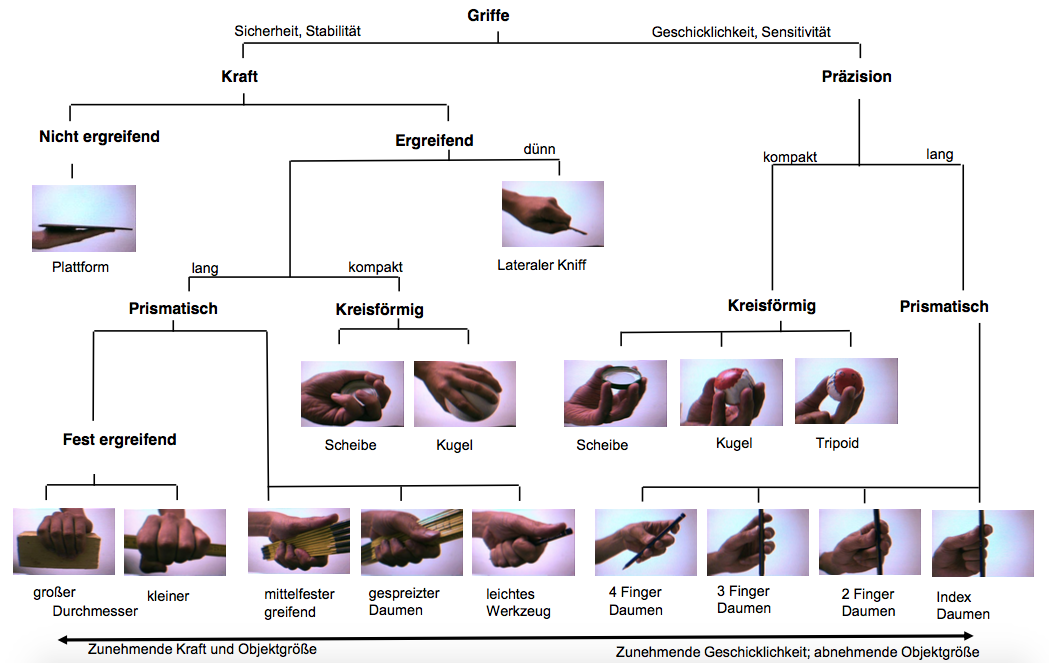
\includegraphics [scale=0.5]{griff}
    \caption{Cutkosky Grifftaxonomie}
\end{figure}

\section{Nebenbedinungen}
\subsection{Intern}
\begin{compactitem}
    \item \textbf{I1: Gültigkeit des Griffes}, Überlappung zwischen den Greifmerkmalen des zu greifenden
    Objektes und den Greifmerkmalen der Greiferfinger
    \item \textbf{I2: Kollisionsfreiheit des Griffes}, keine Kollision zwischen Greifer und gegriffenem
    Objekt
    \item \textbf{I3: Zugänglichkeit des Griffes}, der Griff ist für den Greifer kollisionsfrei erreichbar
\end{compactitem}
\subsection{Extern}
\begin{compactitem}
    \item \textbf{E1: Kollisionsfreie Anrückbewegung des Greifers}, keine Kollision zwischen Roboterarm,
    Grifer, benachbarten Objekten und Arbeitsebene
    \item \textbf{E2: Kollisionsfreie Abrückbewegung mit gegriffenem Objekt}, siehe e1
    \item \textbf{E3: Berücksichtigung der Roboterkinematik}, der selektierte Griff liegt im Arbeitsraum
    des Roboters und die korrespondierenden Trajektorien der Anrück und Abrückbewegung können
    können vom Roboter abgefahren werden.
    \item \textbf{E4: Stabilität des Griffes}, sowohl während der Greifbewegung der Greiferfinger als
    auch während der Transferbewegung des Greifers mit gegriffenem Objekt verändert sich die relative
    Lage und Orientierung des zu greifenden/gegriffenen Objekts zum Greifer nicht
    \item \textbf{E5: Stabilität der Szene}, Abrückbewegung des Greifers mit gegriffenem Objekt sollte
    die Stabilität der Szene nicht beeinflussen.
    \item \textbf{E6: Aufgabenabhängigkeit des Griffs}, wird Pick and Place Operation ausgeführt, dann
    muss zur Aufnahme und Ablagekonfiguration des zu greifenden Objektes kompatibler Griff gewählt werden.
    \begin{compactitem}
        \item Kann kein Griff bestimmt werden, der Nebenbedingung erfüllt, muss geeignete Umgreifsequenz
        bestimmt werden.
        \item Erfordert Griff Ausübung von Kraft und Kraftmomenten auf das Objekt, so muss Greifer diese
        Aufbringen können
    \end{compactitem}
\end{compactitem}

\section{Greifanalyse und Synthese}
\mparagraph{Greifanalyse}
\begin{compactitem}
    \item gegeben: Objekt und Menge von Kontaktpunkten
    \item gesucht: Aussagen zur Stabilität des Giffs unter Berücksichtung der Nebenbedinungen.
\end{compactitem}
\mparagraph{Greifsynthese}
\begin{compactitem}
    \item gegeben: Objekt und eine Menge von Nebenbedinungen.
    \item gesucht: Menge von Kontaktpunkten
\end{compactitem}

\section{Kontaktmodelle}
\begin{compactitem}
    \item Kontakt ohne Reibung (existiert nicht)
    \item Kontakt mit Reibung (Kraft wirkt normal als auch tangential zur Fläche)
    \item Soft-Kontakt (Kraft wirkt normal, tangential. Zusätzlich wirken axiale Momente)
\end{compactitem}
Reibungskegel wird kontinuierlich oder mit approximiert mit Polyeder beschrieben

\mparagraph{Wrenchvektor}
Vektor $\vec{w}$ fasst die in einem Kontaktpunkt $\vec{p}_i$ wirkenden Kräfte $f_i$ und Momente
$\tau_i$ mit $i \in \{x,y,z\}$ zusammen. \\
In Abhängigekeit vom Typ des i-ten Kontaktpunktes normalen \textbf{n}, tangentiale Kräft \textbf{t} und
axiale Momente \textbf{$\Theta$}: $^i\vec{w}_n, ^i\vec{w}_t, ^i\vec{w}_\Theta$ bzw. korrespondierende
Skalare $^ic_n, ^ic_t, ^ic_\Theta$
\mparagraph{Greifmatrix}
Darstellung der Wrenchvektoren für einen räumlichen Griff als Spaltenvektor einer 6 x 3m Matrix G.

\mparagraph{Gleichgewichtsgriff}
Ein Griff wird als Gleichgewichtsgriff bezeichne,t wenn die Summer aller Kräfte $f_i$ und Momente
$\tau_i$, die auf das gegriffene Objekt wirken, gleich Null ist.
\begin{align}
    &1. \forall i \in \{1, ...,m\} : ^ic_n \geq 0, ^i\mu_t * ^ic_n \geq |^ic_t|, ^i\mu_\Theta * ^ic_n
    \geq |^ic_\Theta| \\
    &2. \exists \vec{c} \in R^{3m}, \vec{c} \neq \vec{0} : G.\vec{c} + \vec{e} = 0
\end{align}
$^i\mu_t, ^i\mu_\Theta \in R$ = Coulombschen Reibungskoeffizienten am i-ten Kontaktpunkt

\section{Kraft und Formgeschlossene Griffe}

% !TEX root = rob1.tex
\chapter{Umweltmodellierung}

\section{Objektmodelle}
\subsection{Kantenmodelle}
\begin{compactitem}
    \item Nur die Kanten werden gespeichert, d.h. Punkte und Verbindungen (Geraden, Polygonzug, Bezierkurve)
    \item \textbf{Vorteile}:
    \begin{compactitem}
        \item einfache Daten
        \item wenige Daten
    \end{compactitem}
    \item \textbf{Nachteile}:
    \begin{compactitem}
        \item Mehrdeutigkeiten
        \item hoher Eingabeaufwand
        \item keine Kollisionsberechnung
        \item kein Schnitt
    \end{compactitem}
\end{compactitem}
\subsection{Flächenmodelle}
\begin{compactitem}
    \item Speicherung von Kanten und Oberflächen (Dreiecke, Bezier)
    \item \textbf{Vorteile}:
    \begin{compactitem}
        \item effiziente Verfahren
        \item entspricht dem Vorgehen während der Modellierung
        \item schnelle Kollisions und Abstandsberechnung
    \end{compactitem}
    \item \textbf{Nachteile}:
    \begin{compactitem}
        \item hoher Eingabeaufwand
        \item Darstellung aufwendig
        \item Problem bei Schnittoperationen
        \item Inkonsitenz möglich
    \end{compactitem}
\end{compactitem}

\mparagraph{Boundary Representation}
Hierarchische Darstellung eines Objektes durch begerenzte Elemente i.d.R Kanten oder Flächen. \\
Beispiel: Elemente eines Quaders im Flächenmodell
\begin{compactitem}
    \item $Q$: Quader
    \item $F_i : i \in \{1,...,6\}$: Flächen
    \item $K_i : i \in \{1,...,12\}$: Kanten
    \item $P_i : i \in \{1,...,8\}$: Ecken
\end{compactitem}
Darstellung in einer topologischen Struktur. Liefert Information über:
\begin{compactitem}
    \item Welche Flächen gehören zum Objekt
    \item Welche Kanten gehören zur Fläche
    \item Zu welchem Objekt gehört eine Kante
    \item Zu welchem Objekt gehört eine Fläche
    \item Welche Flächen stoßen aneinandern?
\end{compactitem}
\subsection{Volumenmodelle}
\subsubsection{A. Punktwolken}
\begin{compactitem}
    \item einfachstes Objektmodell
    \item Modell ist eine beliebige Menge aus Raumpunkten
    \item Daten direkt aus aktuellen Tiefensensoren
    \item Objekt nur implizit, indirekt modelliert
    \item Mehrdeutigkeit
\end{compactitem}
\subsubsection{B. Approximative Oberflächen}
\begin{compactitem}
    \item Bildung einer großen Fläche aus einem Netz von einfachen Einzelflächen
    z.B Dreiecke, Vierecke
    \item \textbf{Vorteile}
    \begin{compactitem}
        \item Definition sehr einfach
        \item einfache Algorithmen
    \end{compactitem}
    \item \textbf{Nachteile}
    \begin{compactitem}
        \item hoher Speicherbedarf
        \item hoher Rechenaufwand
    \end{compactitem}
\end{compactitem}
\mparagraph{Dreiecksfläche}
Approximation von Freiformflächen. Gegeben sind 3 Punkte im Raum $P_1, P_2, P_3$. Dann gilt für die
Fläche: $F(u,v) = u \cdot P_1 + v \cdot P_2 + (1-u-v) \cdot P_3$ mit $0 \leq u,v,u+v \leq 1$
\mparagraph{Bilineare Vierecksflächen}
Fläche ist wie folgt definiert bei 4 gegebenen Punkten im Raum: $F(u,v) = (1-u)(1-v) \cdot P_1 +
(1-u)v \cdot P_2 + u(1-v) \cdot P_3 + uv \cdot P_4$ mit $0 \leq u \leq 1, 0 \leq v \leq 1$
\begin{compactitem}
    \item \textbf{Vorteile}: Flächen können gekrümmt sein. Somit weniger Gitterpunkte bei gleich guter
    Approximation
    \item \textbf{Nachteile}: Rechnen mit gekrümmten Flächen ist aufwendig
\end{compactitem}

\mparagraph{Bezierflächen}
Erweiterung des Ansatzes der Bezierkurven. Gegeben ist ein Gitter mit Führungspunkten $P_{ij},
0 \leq i \leq N$ und $0 \leq j \leq M$
\begin{align}
    F(u,v) &= \sum_{i=0}^N\sum_{j=0}^M  P_{ij} \cdot B_{i,N}(u) \cdot B_{j,M}(v) \\
    B_{i,N}(u) &= (1-u)B_{i,N-1}(u) + u \cdot B_{i-1,N-1}(u)  \\
    B_{j,M}(v) &= (1-v)B_{j,M-1}(v) + v \cdot B_{j-1,M-1}(v)
\end{align}
\subsubsection{Approximative Zellenbelegung}
\mparagraph{A. Voxel}
Objekte werden aus disjunkten Elementarzellen aufgebaut. (Tetraeder, Quader)
\begin{compactitem}
    \item \textbf{Vorteile}:
    \begin{compactitem}
        \item Einfache Darstellung
        \item Berechnung homogen, parallel auf GPU
        \item Raycasting u.ä einfach parallelisierbar
    \end{compactitem}
    \item \textbf{Nachteile}:
    \begin{compactitem}
        \item Festes Gitter, gleicher Detaillierungsgrad sowohl bei großflächigen als auch feiner
        aufgelösten Strukturen
        \item Kartengröße/Präzision durch Speicher begrenzt
    \end{compactitem}
\end{compactitem}
\mparagraph{B. Octree}
\begin{compactitem}
    \item Raum wird in mehrere Zellen unterteilt
    \item Zelle komplett vom Objekt belegt $\rightarrow$ als belegt markieren
    \item Zelle teilweise belegt, dann weiter unterteilen und wiederholen, sonst leer
    \item Rekursion terminiert bei einer vorbestimmten minimalen Zellgröße
    \item Teilbelegt kleinste Zellen werden als belegt markiert
\end{compactitem}
\subsubsection{Analytisch Paramterische Modelle}
Grundkörper und topologische Operationen auf diesen werden abgespeichert. \\
\begin{compactitem}
    \item \textbf{Vorteile}:
    \begin{compactitem}
        \item Eindeutige Objektbeschreibung
        \item Geringer Eingabeaufwand
        \item Ergebnis vo Operationen sind korrekte Objekte
    \end{compactitem}
    \item \textbf{Nachteile}:
    \begin{compactitem}
        \item hoher Implementierungsaufwand
        \item Einbindung von Freiformflächen schwierig
    \end{compactitem}
\end{compactitem}
\mparagraph{Constructive Solid Geometrz, CSG}
Objekte sind bereits vorhanden und können durch Angabe von Parametern angepasst werden (Varianten) z.B
\begin{compactitem}
    \item \textbf{Körper}
    \begin{compactitem}
        \item \textbf{Quader}: Länge, Breite, Höhe
        \item \textbf{Prisma}: Länge, Radius, Facettem
        \item \textbf{Zylinder}: Länge Radius
        \item \textbf{Kegel}: Länge, Radius a, Radius b
        \item \textbf{Ellipsoid}: Radius a, Radius b, Radius c
    \end{compactitem}
    \item \textbf{Operatoren}
    \begin{compactitem}

        \item \textbf{Vereinigung}: $A \cup B$
        \item \textbf{Schnitt}: $A \cap B$
        \item \textbf{Differenz}: $A / B$
        \item \textbf{Sweep}: Ein Grundelement wird entlang einer Raumkurve geschoben. Der durchdrungene
        Raum stellt das neue Objekt dar.
        \item Speicherung erfolgt als Binärbaum mit Knoten als Operation und Teilbaum als Teil-CSG oder
        Grundkörper
    \end{compactitem}
\end{compactitem}

\section{Umwandlung}
\begin{figure}[!h]
    \centering
    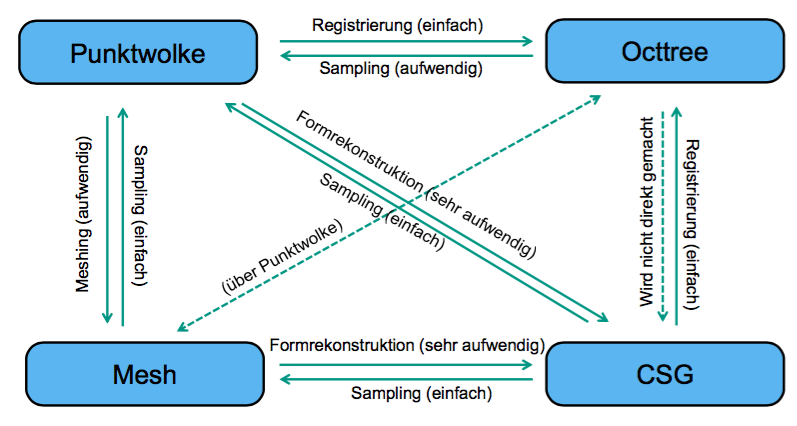
\includegraphics [scale=0.5]{umwandlung}
\end{figure}

% !TEX root = rob1.tex
\chapter{Interaktive Programmierung}

% !TEX root = rob1.tex
\chapter{ARMAR}

 \section{Greifen}
 \subsection{Offline Grasp Analyse}
 \begin{compactitem}
     \item Durchführbahre Griffe werden für jedes Objekt offline berechnet und
     zusammen mit dem Objektmodell gespeichert
     \item Griff ist definiert durch
     \begin{compactitem}
         \item Grasping Center Point des Objekts der mit dem TCP auf einer Linie
         ist
         \item Approach Vector, beschreibt den Winkel in dem die Hand den Greifpunkt
         anfährt
         \item Wrist Orientation
         \item Initial Finger Configuration
     \end{compactitem}
 \end{compactitem}

 \subsection{Objekt Klassen}
 \subsubsection{Bekannte Objekte}
 \begin{compactitem}
     \item Objektgeometrie bekannt
     \item Verwende bekannte Greifplanungsmethoden für bekannte Objekte
     \item Hard
 \end{compactitem}
 \subsubsection{Verwandte Objekte}
 \begin{compactitem}
     \item Klasse des Objekts ist bekannt, z.B Flasche
     \item Wiederverwendung von Greifwissen für bekannte Klassenmitglieder auf
     neues Objekt
     \item Harder
 \end{compactitem}
 \subsubsection{Unbekannte Objekte}
 \begin{compactitem}
     \item Kein Wissen über Objekt vorhanden
     \item Herausforderung: Arbeiten mit (unvollständigen) Sensordaten (Stereovision,
     RGB-D, Laser Scan, Haptische Daten...), Trennung/Segentierung vom Hintergrund und
     Bau eines (Teil)Objektmodells
     \item Hardest!
 \end{compactitem}

 \subsection{Grasping by parts / part-based grasping}
 \begin{compactitem}
     \item Idee ist Objekte in einfache Teile aufzulösen.
     \item Plane Griffe für einzelne Segmente
 \end{compactitem}
 Forward-Ansatz der Planung
 \begin{compactitem}
     \item Führe Hand an Objekt bis Kollision
     \item Schließe finger um Objekt bis Kollision
     \item Evaluiere Kontakt von Hand und Objekt. Ist der Griff ,,force-closure''
     oder nicht
 \end{compactitem}


 \section{Box Decomposition Algorithm}
 \subsection{Von Punkten zu Boxen}
 \begin{compactitem}
     \item Nimm eine Punktwolke und bestimte Minimum Volume Bounding Box mit
     $O(n log n + n/\epsilon^3)$
     \item Es wird ein Aufspaltungs Kriterium benötigt, welches die haupt MVBB in
     eine menge kleinere Boxen aufteilt, welche die Form detaillierter darstellen
     \item Teile Form in semantische Teile auf z.B Kopf und Körper
     \item Benutze Flächen, die parallel zur Eltern MVBB ist
     \item Ein Split einer Parentbox ist besser, je weniger Volumen die resultierenden
     Kinder beinhalten
 \end{compactitem}

\subsection{Von Boxen zu Griffen}
\item Jede Box hat 6 Seiten welche ein Set von intuitiven Greifhypothesen liefern:
Entlang dem Zentrum, oder entlang der Normale
\item Die Facedimension kann benutzt werden, umm Greifhypothesen abzuweisen, die
größer als die Handöffnung sind
\item Für jede Seite kann ohne weiters 4 Hypothesen, welche sich in der Handorientierung
unterscheiden, erzeugen
\item Blockierte oder verdeckte Seiten können einfach ausgeschlossen werden durch
geometrische Berechnungen

\section{Medial Axis}
\begin{compactitem}
    \item Repräsentieren das topologische Skelet eines Objektes
    \item Die Medial Axis ist eine Formapproximation eines Objekte mit Hilfe von
     Sphären maximalen Durchmessers.
    \item Sphären müssen die Geometrische Form von innen an min. 2 Punkten berühren
    \item Medial Axsis ist als Vereinigung aller Sphärenzentren definiert

\end{compactitem}
\mparagraph{Vorteile}
\begin{compactitem}
    \item Gute Approximation der Objektgeometrie
    \item Details bleiben erhalten
    \item Symmetrische Eigenschaften eines Objektes können aus den Medial Axis
    extrahiert werden
    \item Einfach um Greifplanung zu evaluieren
\end{compactitem}

\subsection{Algorithmus zur identifizierung von Slices einer Medial Axis}
\begin{compactenum}
    \item Minimum Spanning Tree der Sphären Zentren in der Ebene
    \item Lösche Kanten die länger sind als Schwellwert
    \item Clustere die entstandenen Bäume und führe für jedes Cluster aus:
    \begin{compactitem}
        \item Bestimme Volumen der Konvexen Hülle
        \item Bestimme Randpunkte der Konvexen Hülle
        \item Bestimmte Zweigknoten (Knoten mit Anzahl Kanten > 2)
        \item Bestimmte Zentrum der Gravity
    \end{compactitem}
\end{compactenum}

% !TEX root = rob1.tex
\chapter{Bildverarbeitung}

\section{Bildrepräsentation}
\textbf{Ein Bild ist ein 2D Gitter von diskreten Punkten (Pixel)}

\mparagraph{Koordinaten}
\begin{compactitem}
    \item $u$, horizontal
    \item $v$, vertikal
    \item Ursprung ist oben links
\end{compactitem}


\section{Farbmodelle}
\mparagraph{Graustufenbild}
Für jeden Pixel wird ein Helligkeitswert abgelegt. Normalerweise 1 Byte pro Pixel
[0,255]

\mparagraph{Monochrombild}
Diskrete Funktion
\begin{align}
    &\text{IMG}:[0..n-1] \times [0..m-1] \rightarrow [0..q]
    &(u,v) \rightarrow \text{Img}(u,v)
\end{align}

\mparagraph{Farbbild}
Verschiedene Farbmodelle für unterschiedliche Anwendungen.
\begin{compactitem}
    \item RGB
    \item HSI: geeignet für Farbsegmentierung
    \item CIE: Physikalisch
    \item CMYK: Substraktive Farbmischung
    \item YIQ
\end{compactitem}

\subsection{RGB}
\begin{compactitem}
    \item Additive Farbmischung
    \item Rot, Grün, Blau
    \item RGB24: ein Pixel durch 3 Bytes dargestellt
\end{compactitem}
\subsection{HSI}
\begin{compactitem}
    \item Hue, Saturation und Intensity/Value
    \item Trenning von Helligkeit vom Farbwert $\rightarrow$ unempfindlich gegen
    Beleuchtungsänderungen
    \item Umrechung RGB nach HSI
    \begin{compactitem}
        \item H undefiniert falls R = G = B
        \item S undefiniert falls R = G = B = 0
    \end{compactitem}
\end{compactitem}
\begin{align}
    H &= \begin{cases} \Theta, \text{ falls } B < G \\ 360 - \Theta, \text{ sonst}
        \end{cases} \\
    \Theta &= \arccos\frac{2R-G-B}{2\sqrt{(R-G)^2 + (R+B)(G-B)}} \\
    S &= 1 - \frac{3}{R + G + B}\min(R,G,B) \\
    I &= \frac{1}{3}(R+G+B)
\end{align}

\section{Lochkamera}
Projektion eines Szenenpunkt $(x,y,z)$ auf einen Bildpunkt $(u,v)$
\begin{align}
    \begin{pmatrix}u \\ v \end{pmatrix} &= \frac{f}{z} \begin{pmatrix} x \\ y \end{pmatrix} \\
    \begin{pmatrix}x \\ y \end{pmatrix} &= \frac{z}{f} \begin{pmatrix}u \\ v \end{pmatrix}
\end{align}

\section{Filteroperationen}
\subsection{Tiefpassfilter}
\textbf{Glättung, Rauschelimination}
\subsubsection{Mittelwertfilter}
\begin{displaymath}
     \begin{pmatrix}
         \frac{1}{9} & \frac{1}{9} & \frac{1}{9} \\
         \frac{1}{9} & \frac{1}{9} & \frac{1}{9} \\
         \frac{1}{9} & \frac{1}{9} & \frac{1}{9}
     \end{pmatrix}
\end{displaymath}
\subsubsection{Gauss Filter}
Ortsbereich: $ f(x,y) = \frac{1}{2\pi\sigma^2}e^{-\frac{x^2+y^2}{2\sigma^2}}$\\
Frequenzbereich:$ F(u,v) = e^{-\frac{u^2+v^2}{2}\sigma^2} $\\
Approximation von f(x) durch 3x3 Filter mit $\sigma = 0.85$
\begin{displaymath}
     F_\text{Gauss} = \frac{1}{16} \begin{pmatrix}
         1 & 2 & 1 \\ 2&4&2\\1&2&1
 \end{pmatrix}
\end{displaymath}
Je größer $\sigma$, desto stärker die Glättung
\subsection{Hochpassfilter}
\textbf{Kantendetektion}

\subsubsection{Prewitt}
\begin{align}
    P_x &= \begin{pmatrix}-1&0&1\\-1&0&1\\-1&0&1 \end{pmatrix}
    P_y &= \begin{pmatrix}-1&-1&-1\\0&0&0\\1&1&1 \end{pmatrix}
\end{align}
Kombination der Prewitt Filter zur Bestimmung des Gradientenbetrags M
\begin{displaymath}
     M \approx \sqrt{{P_x}^2 + {P_y}^2}
\end{displaymath}
Danach Schwellwertfilterung

\section{Segmentierung}
\textbf{Aufteilung eines Bildes in aussagekräftige Segmente}
\subsection{Schwellwertfilterung}
Konvertierung eines Grauwertbildes in ein binäres Bild. \\
Generell können Objekte über ihre Farbe segmentiert werden. \\
Problematisch sind wechselnde Lichtbedinungen, Reflexionen und Schattenwürfe

\subsection{Morphologische Operatoren}
\subsubsection{Dilatation}
Vergrößert Pixel zu größeren Bereichen \\
Prüfe an jeder Position ob Maske H teilmenge von Bild B ist
\subsubsection{Erosion}
Entfernt einzelne Pixel und schwach zusammenhängende Pixelgruppen \\
Prüfe an jeder Position ob Schnittmenge von Bild B und Maske H nicht leer ist.

\subsection{Canny Kantendetektor}
\begin{compactenum}
    \item Rauschunterdrückung durch Gauss Filter
    \item Kantendetektion mit Sobel oder Prewitt
    \item Non Maximum Supression
    \begin{compactitem}
        \item Gradient muss lokales Max. sein
        \item Betrachtung der zwei direkten Nachbarn entlang der Gradientenrichtung
        \item Überprüfung erfolg gemäß dem jeweiligen Quadranten
    \end{compactitem}
    \item Hysterese Schwellwertverfahren
    \begin{compactitem}
        \item Verwende Schwellwerte low und high
        \item Liegt der Betrag des Gradienten für einen Pixel über high, so wird er
        auf jedenfall akzeptiert
        \item Ausgehen von den akzeptierten Pixel werden Kanten rekursiv verfolg
        \begin{compactitem}
            \item Überprüfung der 8 direkten Nachbarn
            \item Betrag Gradient muss über low liegen
        \end{compactitem}
    \end{compactitem}
\end{compactenum}

\section{Registrierung von Punktwolken mit Iterative Closest Point, ICP}
Registrierung ist die Zusammenführung von Punktwolken, welche das gleiche
Objekt aus unterschiedlichen Ansichten beschreibt

\subsection{Algorithmus}
Registrierung zweier 3D Punktwolken und minimiert Distanz zwischen ihnen

\begin{compactenum}
    \item Für jede Iteration k gilt:
    \begin{compactitem}
        \item Für jeden Punkt $a_i$ aus A suche Punkt $b_i$ aus B, der $a_i$ am nächsten
        liegt.
        \item Berechen eine Transformation $T_k$, so dass $D_k$ minimal wird. z.B
        $D_k = \sum_i || a_i - T_k \cdot b_i || ^2$
    \end{compactitem}
    \item $D_k$ kombiniert Translation und Rotation
    \item Wende Transformatin $T_k$ auf alle Punkte aus B an
    \item Abbrichkriterium: Schwellwert für $D_{k-1}-D_k$ oder max. Iterationen erreicht.
    \item \textbf{Vorteile}:
    \begin{compactitem}
        \item Algorithmus für Punkte, Normalenvektoren und andere Darstellungsformen
        anwendbar
        \item Nur einfache mathematische Operation notwendig
        \item Schnelles Registrierungsergebnis
    \end{compactitem}
    \item \textbf{Nachteile}:
    \item Symmetrische Objekte können nicht ohne wieteres registriert werden
    \item Konvergenz in ein lokales Minimum möglich
    \item Überlappung der Punktwolken erforderlich
\end{compactenum}

\section{Random Sample Consensus, RANSAC}
\begin{compactitem}
    \item \textbf{RANSAC ist ein nicht deterministischer Algorithmus. Ist eine iterative
    Methode zur Schätzung von Modellparametern aus Datenpunkten}
    \item Robust gegenüber Ausreißern und fehlenden Datenpunkten
    \item Anwendung in  Bildverarbeitung
    \begin{compactitem}
        \item Schätzung von Lininen in 2D Bildern
        \item Schätzung vno Ebenen und anderen Primitiven in 3D Punktwolken
    \end{compactitem}
    \item \textbf{Vorteile}:
    \begin{compactitem}
        \item Einfach, allgemein und einfach zu implementieren
        \item Robuste Modellschätzung für Daten mit wenigen Ausreißern
        \item Vielseitig anwendbar
    \end{compactitem}
    \item \textbf{Nachteile}:
    \begin{compactitem}
        \item Nicht Deterministisch
        \item Viele Parameter
        \item Trade off zwischen Genauigkeit und Laufzeit
        \item Nicht anwendbar wenn Verhältnis Inliers/Outliers zu klein ist
    \end{compactitem}
\end{compactitem}

\subsection{Algorithmus}
\begin{compactenum}
    \item Wähle zufällig die min. Anzahl an Punkten aus, die nötig ist um die
    Modellparameter zu berechnen. (2 für Linie in 2D, 3 für Ebene in 3D)
    \item Schätze ein Modell aus dem ausgewählten Datensatz
    \item Bewertung der Modellschätzung: Berechne die Teilmenge der Datenpunkte
    (Inliers), deren Abstand zum Modell kleiner ist als ein vordefinierter Schwellwert
    \item Wiederhole 1-3 bis das Modell mit den meisten Inliers gefunden wird
\end{compactenum}

\section{Normalenschätzung in 3D Punktwolken}
\textbf{Ziel: Zusätzliche Oberflächeninformation durch Einbeziehung lokaler
Nachbarpunkte}. \\
Dient als Grundlage für weiterführende Algorithmen der Segmentierung,
Deskriptoren, Objekterkennung oder Oberflächenmodellierung

\subsection{PCA basierter Ansatz}
\begin{compactitem}
    \item Erstelle die Kovarianzmatrix C der k-Punktnachbarschaft für jeden Punkt p
    \item Bestimme die Eigenwerte und Eigenvektoren von C
    \begin{compactitem}
        \item Hauptkomponentenanalyse
        \item Eigenvektor zu kleinstem Eigenwert korrespondiert mit der Normalen
    \end{compactitem}
\end{compactitem}
\begin{displaymath}
     C = \frac{1}{k}\sum_1^k (p_i - \overline{p})(p_i - \overline{p})^T
\end{displaymath}
\begin{compactitem}
    \item $p_i$ k Nachbarpunkte
    \item $\overline{p}$ Mittelpunkt aller k Nachbarn
\end{compactitem}

\section{Simultaneous Localization and Mapping, SLAM}
\textbf{Slam ist eine Abschätzung von sowohl der Position des Roboters als auch der
Karte der Umgebung zur gleichen Zeit} \\

Slam wird benötigt um voll autonome Roboter zu bauen, um in einer unbekannten
Umgebung überleben zu können, um zu wissen wo sich der roboter befindet und zur
Navigation ohne externe Positionssysteme wie GPS

\subsubsection{Terme}
\begin{compactitem}
    \item \textbf{Localization}: Abschätzung des Aufenthaltsorts des Roboters, gegeben
    eine Karte
    \item \textbf{Mapping}: Ableiten einer Karte gegeben einem Set von Orten
    \item \textbf{SLAM}: Erstelle eine Map und lokalisiere den Roboter zeitgleich!
\end{compactitem}

\subsubsection{Problem}
Man benötigt eine Karte um den Roboter zu lokalisieren, aber zeitgleich die
Positionen des Roboters um eien Karte zu erstellen. \\
$\Rightarrow$ Tracking der Bewegung der Kamera und des Roboters

\subsubsection{Benötigte Features}
\begin{compactitem}
    \item SLAM System, dass Szenenfeatures festhält (Landmarks)
    \item Visuelle Features sind Punkte, Ecken, Linien, Texturen oder Oberflächen
    \item Features müssen beschreibend und eindeutig sein!
\end{compactitem}

\subsubsection{How to do SLAM}
\begin{compactitem}
    \item Verwende Interne Repräsentation für Position der Landmarks und der Kameraparameter
    \item Für jeden Frame (Bewege und schaue):
    \begin{compactitem}
        \item Sage hervor, um wieviel sich der Roboter bewegt hat
        \item Halte neue Landmarks fest
        \item Update die interne Repräsentation durch die Messunsicherheiten
    \end{compactitem}
    Wenn Roboter alten Landmark erkennt: Loop closing!
\end{compactitem}




\end{document}
